
\subsection{Suffix Arrays and Suffix Trees}

\begin{figure*}[phbt]
\begin{subfigure}[t]{0.5\textwidth}
\centering
%\scalebox{0.9}{

\tikzstyle{leaf}=[draw=red!90,fill=red!40,rectangle,thick,minimum height=2.6ex,minimum width=2ex,inner sep=0pt]
\tikzstyle{internal}=[fill=black,circle,inner sep=0pt,minimum size=1ex]

\def\yscale{0.6}
\def\xscale{0.7}

\begin{tikzpicture}
% \draw [help lines] (0,0) grid (10,10);
% \node at (0,0) {(0,0)};
% \node at (10,0) {(10,0)};
% \node at (0,10) {(0,10)};
% \node at (10,10) {(10,10)};

\node[internal] (root) at (5*\xscale,10*\yscale) {};

% children of the root
\node[leaf] (leaf-0) at (0*\xscale,9*\yscale) {\small$22$};
\node[internal] (root-subtree-0) at (1*\xscale,8.5*\yscale) {};
\node[internal] (root-subtree-1) at (2*\xscale,8*\yscale) {};
\node[internal] (root-subtree-2) at (3.2*\xscale,7.6*\yscale) {};
\node[internal] (root-subtree-3) at (4*\xscale,7*\yscale) {};
\node[internal] (root-subtree-4) at (4.5*\xscale,6*\yscale) {};
\node[internal] (root-subtree-5) at (5.7*\xscale,6.9*\yscale) {};
\node[leaf] (leaf-15) at (6.5*\xscale,8*\yscale) {\small$2$};
\node[internal] (root-subtree-6) at (8*\xscale,8.7*\yscale) {};
\node[leaf] (leaf-22) at (10*\xscale,9*\yscale) {\small$10$};

%children of root-subtree-0
\node[leaf] (leaf-1) at (0.1*\xscale,8*\yscale) {\small$21$};
\node[internal] (subtree-0-subtree-1) at (0.5*\xscale,7*\yscale) {};

%children of subtree-0-subtree-1
\node[leaf] (leaf-2) at (0.25*\xscale,5*\yscale) {\small$11$};
\node[leaf] (leaf-3) at (0.7*\xscale,4*\yscale) {\small$0$};

% %children of root-subtree-1
\node[leaf] (leaf-4) at (1.2*\xscale,7*\yscale) {\small$18$};
\node[leaf] (leaf-5) at (1.3*\xscale,1.75*\yscale) {\small$8$};

% %children of root-subtree-2
\node[leaf] (leaf-6) at (2.2*\xscale,6.7*\yscale) {\small$17$};
\node[leaf] (leaf-7) at (2.4*\xscale,3*\yscale) {\small$7$};

% %children of root-subtree-3
\node[leaf] (leaf-8) at (3.3*\xscale,5.5*\yscale) {\small$14$};
\node[leaf] (leaf-9) at (3.5*\xscale,1.6*\yscale) {\small$4$};

% %children of root-subtree-4
%\node[leaf] (leaf-10) at (4.3*\xscale,5.5*\yscale) {\small$20$};
%\node[internal] (subtree-4-subtree-1) at (4.8*\xscale,4*\yscale) {};

% %children of subtree-4-subtree-1
\node[leaf] (leaf-10) at (3.9*\xscale,2.5*\yscale) {\small$15$};
\node[leaf] (leaf-11) at (4.7*\xscale,1.5*\yscale) {\small$5$};

% %children of root-subtree-4
\node[leaf] (leaf-12) at (5.1*\xscale,6*\yscale) {\small$20$};
\node[internal] (subtree-5-subtree-1) at (5.7*\xscale,5*\yscale) {};
\node[leaf] (leaf-13) at (5.5*\xscale,2.5*\yscale) {\small$13$};
\node[leaf] (leaf-14) at (6.2*\xscale,1.5*\yscale) {\small$3$};

% %children of root-subtree-5
% \node[leaf] (leaf-9) at (3.5,2.5*\yscale) {\small$18$};
% \node[internal] (subtree-5-subtree-1) at (4,2*\yscale) {};

% %children of subtree-5-subtree-1
% \node[leaf] (leaf-10) at (3.6,0.5*\yscale) {\small$11$};
% \node[leaf] (leaf-11) at (4.1,0*\yscale) {\small$2$};

% %children of root-subtree-6

\node[internal] (subtree-6-subtree-1) at (7.5*\xscale,6*\yscale) {};
\node[internal] (subtree-6-subtree-2) at (8.5*\xscale,5.5*\yscale) {};
\node[leaf] (leaf-16) at (6.7*\xscale,4.5*\yscale) {\small$16$};
\node[leaf] (leaf-17) at (7.7*\xscale,1.5*\yscale) {\small$6$};

\node[leaf] (leaf-18) at (8.4*\xscale,3.5*\yscale) {\small$19$};
\node[leaf] (leaf-19) at (9*\xscale,1.5*\yscale) {\small$12$};
\node[leaf] (leaf-20) at (9.2*\xscale,6.5*\yscale) {\small$1$};
\node[leaf] (leaf-21) at (9.8*\xscale,7.5*\yscale) {\small$9$};


% edge label mapping
% #           1
% the 1       8
% old 2       7
% night 3     6
% keeper 4    4
% keeps 5     5
% keep 6      3
% in 7        2
% town 8      9
% 
% # 
% 1876458328918645832861

% edges from root to children
\draw (root) -- (leaf-0.north)  node [midway,above=-3pt,sloped] {\tiny \tt \$};
\draw (root) -- (root-subtree-0)  node [sloped,midway,above=-3pt] {\tiny \tt \#};
\draw (root) -- (root-subtree-1)  node [sloped,midway,above=-3pt] {\tiny \tt the in};
\draw (root) -- (root-subtree-2)  node [sloped,midway,above=-3pt] {\tiny \tt in keep};
\draw (root) -- (root-subtree-3)  node [sloped,midway,above=-3pt] {\tiny \tt ..keeper};
\draw (root) -- (root-subtree-4)  node [sloped,midway,above=-3pt] {\tiny \tt keeps};
\draw (root) -- (root-subtree-5)  node [sloped,midway,above=-3pt] {\tiny \tt night};
\draw (root) -- (leaf-15.north)  node [sloped,midway,above=-3pt] {\tiny \tt old..\$};
\draw (root) -- (root-subtree-6)  node [sloped,midway,above=-3pt] {\tiny \tt the};
\draw (root) -- (leaf-22.north)  node [midway,above=-3pt,sloped] {\tiny \tt town..\$};

% edges from root-subtree-1 to children
\draw (root-subtree-0) -- (leaf-1.north)  node [midway,above=-3pt,sloped] {\tiny \tt \$};
\draw (root-subtree-0) -- (subtree-0-subtree-1)  node [midway,above=-3pt,sloped] {\tiny \tt the};

% edges from subtree-0-subtree-1 to children
\draw (subtree-0-subtree-1) -- (leaf-2.north)  node [midway,above=-3pt,sloped] {\tiny \tt \$..night};
\draw (subtree-0-subtree-1) -- (leaf-3.north)  node [sloped,midway,above=-3pt] {\tiny \tt old night..\$};

% % edges from root-subtree-1 to children
\draw (root-subtree-1) -- (leaf-4.north)  node [midway,above=-3pt,sloped] {\tiny \tt \$\#night};
\draw (root-subtree-1) -- (leaf-5.north)  node [midway,above=-3pt,sloped] {\tiny \tt \$..keeper night the \#town};

% % edges from root-subtree-2 to children
\draw (root-subtree-2) -- (leaf-6.north)  node [midway,above=-3pt,sloped] {\tiny \tt \$\#night};
\draw (root-subtree-2) -- (leaf-7.north)  node [midway,above=-3pt,sloped] {\tiny \tt ..night the town};

% % edges from root-subtree-3 to children
\draw (root-subtree-3) -- (leaf-8.north)  node [midway,above=-3pt,sloped] {\tiny \tt \$\#night};
\draw (root-subtree-3) -- (leaf-9.north)  node [midway,above=-3pt,sloped] {\tiny \tt ..the town};

% % edges from root-subtree-4 to children
%\draw (root-subtree-4) -- (leaf-10.north)  node [midway,above=-3pt,sloped] {\tiny \tt \$\#};
%\draw (root-subtree-4) -- (subtree-4-subtree-1)  node [midway,above=-3pt,sloped] {\tiny \tt the in keep the};

% % edges from root-subtree-4 to children
\draw (root-subtree-4) -- (leaf-10.north)  node [midway,above=-3pt,sloped] {\tiny \tt \$\#night};
\draw (root-subtree-4) -- (leaf-11.north)  node [sloped,midway,above=-3pt] {\tiny \tt town\# the night..};

% % edges from subtree-5-subtree-1 to children
\draw (root-subtree-5) -- (leaf-12.north)  node [midway,above=-3pt,sloped] {\tiny \tt \$\#};
\draw (root-subtree-5) -- (subtree-5-subtree-1)  node [midway,above=-3pt,sloped] {\tiny \tt keeper..};
\draw (subtree-5-subtree-1) -- (leaf-13.north)  node [midway,above=-3pt,sloped] {\tiny \tt \$\#night};
\draw (subtree-5-subtree-1) -- (leaf-14.north)  node [sloped,midway,above=-3pt] {\tiny \tt town\# the..\$};


% % edges from root-subtree-6 to children
% \draw (root-subtree-6) -- (leaf-17.north)  node [sloped,midway,above=-3pt] {\tiny \tt old..\$};
% \draw (root-subtree-6) -- (leaf-18.north)  node [sloped,midway,above=-3pt] {\tiny \tt town..\$};
\draw (root-subtree-6)  -- (subtree-6-subtree-1)  node [sloped,midway,above=-3pt] {\tiny \tt the in keep};
\draw (root-subtree-6)  -- (subtree-6-subtree-2)  node [sloped,midway,above=-3pt] {\tiny \tt night};
\draw (subtree-6-subtree-2) -- (leaf-18.north)  node [midway,above=-3pt,sloped] {\tiny \tt \$\#};
\draw (subtree-6-subtree-2) -- (leaf-19.north)  node [midway,above=-3pt,sloped] {\tiny \tt keeper keeps..\$};
\draw (root-subtree-6) -- (leaf-20.north)  node [midway,above=-3pt,sloped] {\tiny \tt old..\$};
\draw (root-subtree-6) -- (leaf-21.north)  node [midway,above=-3pt,sloped] {\tiny \tt town..\$};
% \draw (root-subtree-6)  -- (subtree-6-subtree-2)  node [sloped,midway,above=-3pt] {\tiny \tt night};

% % edges from root-subtree-subtree-6-subtree-1 to children
\draw (subtree-6-subtree-1)  -- (leaf-16.north)  node [sloped,midway,above=-3pt] {\tiny \tt \$\#night};
\draw (subtree-6-subtree-1)  -- (leaf-17.north)  node [sloped,midway,above=-3pt] {\tiny \tt town\# the night..\$};


% % edges from root-subtree-subtree-6-subtree-2 to children
% \draw (subtree-6-subtree-2)  -- (leaf-15.north)  node [sloped,midway,above=-3pt] {\tiny \tt \$};
% \draw (subtree-6-subtree-2)  -- (leaf-16.north)  node [sloped,midway,above=-3pt] {\tiny \tt keeper..\$};


\matrix[
  matrix of nodes,
  nodes={
    draw,
    minimum height=2ex,
    minimum width=1.5ex,
    inner sep=1pt,
    font=\fontsize{7}{8}\selectfont,
    align=center
    }
  ]
 (mat) at (3.4,0)
 {
 22 & 21 & 11 & 0 & 18 & 8 & 17 & 7 & 14 & 4 & 15 & 5 & 20 & 13 & 3 & 2 & 16 & 6 & 19 & 12 & 1 & 9 & 10 \\
 };

%\node[left of=mat,node distance=3.7cm] {\SA};

\end{tikzpicture}
%}
\caption{Word-based Suffix Tree.}
\label{fig-suffix-tree}
\end{subfigure}
\quad
\begin{subfigure}[t]{0.5\textwidth}
\centering
\tikzstyle{internal}=[draw,rectangle,inner sep=0pt,minimum size=1ex,align=center]
\tikzstyle{leaf}=[draw,rectangle,fill=blue!50,inner sep=0pt,minimum size=1ex,minimum height=15pt,align=center]

\def\yscale{0.9}
\def\xscale{1}

\def\lvlzero{9.5}
\def\lvlone{8.1}
\def\lvltwo{6.8}
\def\lvlthree{5.5}
\def\lvlfour{4.3}

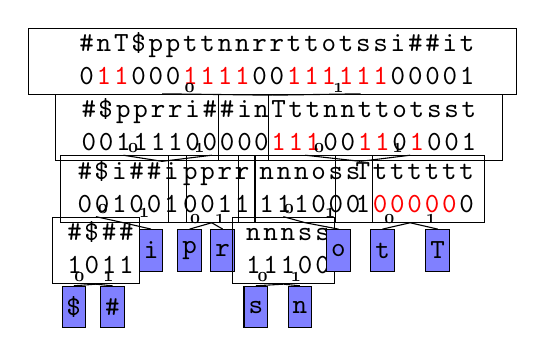
\begin{tikzpicture}

\node[internal,text width=6.2cm] (root) at (5*\xscale,\lvlzero*\yscale) {
\setlength\tabcolsep{0.5pt}
\begin{tabular}{ccccccccccccccccccccccc}
{\tt \#} & {\tt n} & {\tt T} &{\tt \$} &{\tt p} &{\tt p} &{\tt t} &{\tt t} &{\tt n} &{\tt n} 
&{\tt r} &{\tt r} &{\tt t} &{\tt t} &{\tt o} &{\tt t} &{\tt s} &{\tt s}&{\tt i}
&{\tt \#}&{\tt \#}&{\tt i}&{\tt t} \\
{\tt 0} & {\tt \color{red}{1}} & {\tt \color{red}{1}} &{\tt 0} &{\tt 0} &{\tt 0} &{\tt \color{red}{1}} &{\tt \color{red}{1}} &{\tt \color{red}{1}} &{\tt \color{red}{1}}
&{\tt 0} &{\tt 0} &{\tt \color{red}{1}} &{\tt \color{red}{1}} &{\tt \color{red}{1}} &{\tt \color{red}{1}} &{\tt \color{red}{1}} &{\tt \color{red}{1}}&{\tt 0}
&{\tt 0}&{\tt 0}&{\tt 0}&{\tt 1} \\
\end{tabular}
};

\node[internal,text width=2.7cm] (n-hdppri) at (3*\xscale,\lvlone*\yscale) {
\setlength\tabcolsep{0.5pt}
\begin{tabular}{cccccccccc}
{\tt \#} &{\tt \$} &{\tt p} &{\tt p} &{\tt r} &{\tt r} &{\tt i}&{\tt \#}&{\tt \#}&{\tt i} \\
{\tt 0} &{\tt 0} &{\tt 1} &{\tt 1} &{\tt 1} &{\tt 1} &{\tt 0}&{\tt 0}&{\tt 0}&{\tt 0}
\end{tabular}
};

\node[internal,text width=3.6cm] (n-ntTos) at (6.6*\xscale,\lvlone*\yscale) {
\setlength\tabcolsep{0.5pt}
\begin{tabular}{cccccccccccccc}
{\tt n} & {\tt T} &{\tt t} &{\tt t} &{\tt n} &{\tt n} &{\tt t} &{\tt t} &{\tt o} &{\tt t} &{\tt s} &{\tt s}&{\tt t} \\
{\tt 0} & {\tt \color{red}{1}} &{\tt \color{red}{1}} &{\tt \color{red}{1}} &{\tt 0} &{\tt 0} &{\tt \color{red}{1}} &{\tt \color{red}{1}} &{\tt 0} &{\tt \color{red}{1}} &{\tt 0} &{\tt 0}&{\tt 1} \\
\end{tabular}
};

\node[internal,text width=1.6cm] (n-hashidollar) at (2.3*\xscale,\lvltwo*\yscale) {
\setlength\tabcolsep{0.5pt}
\begin{tabular}{cccccc}
{\tt \#} &{\tt \$} &{\tt i}&{\tt \#}&{\tt \#}&{\tt i} \\
{\tt 0} &{\tt 0} &{\tt 1} &{\tt 0}&{\tt 0}&{\tt 1}
\end{tabular}
};

\node[internal,text width=1.1cm] (n-pr) at (3.9*\xscale,\lvltwo*\yscale) {
\setlength\tabcolsep{0.5pt}
\begin{tabular}{cccc}
{\tt p} &{\tt p} &{\tt r}&{\tt r}  \\
{\tt 0} &{\tt 0} &{\tt 1}&{\tt 1}
\end{tabular}
};

\node[leaf,text width=0.3cm] (l-p) at (3.5*\xscale,\lvlthree*\yscale) {
{\tt p}
};

\node[leaf,text width=0.3cm] (l-r) at (4.1*\xscale,\lvlthree*\yscale) {
{\tt r}
};

\node[internal,text width=1.1cm] (n-hashdollar) at (1.8*\xscale,\lvlthree*\yscale) {
\setlength\tabcolsep{0.5pt}
\begin{tabular}{cccc}
{\tt \#} &{\tt \$} &{\tt \#}&{\tt \#}  \\
{\tt 1} &{\tt 0} &{\tt 1}&{\tt 1}
\end{tabular}
};

\node[leaf,text width=0.3cm] (l-i) at (2.8*\xscale,\lvlthree*\yscale) {
{\tt i}
};

\node[leaf,text width=0.3cm] (l-dollar) at (1.4*\xscale,\lvlfour*\yscale) {
{\tt \$}
};

\node[leaf,text width=0.3cm] (l-hash) at (2.1*\xscale,\lvlfour*\yscale) {
{\tt \#}
};


\node[internal,text width=1.7cm] (n-nso) at (5.6*\xscale,\lvltwo*\yscale) {
\setlength\tabcolsep{0.5pt}
\begin{tabular}{cccccc}
{\tt n} & {\tt n} &{\tt n} &{\tt o} &{\tt s} &{\tt s}\\
{\tt 1} & {\tt 1} &{\tt 1} &{\tt 0} &{\tt 0} &{\tt 0} \\
\end{tabular}
};

\node[internal,text width=1.9cm] (n-tT) at (7.5*\xscale,\lvltwo*\yscale) {
\setlength\tabcolsep{0.5pt}
\begin{tabular}{ccccccc}
{\tt T} & {\tt t} &{\tt t} &{\tt t} &{\tt t} &{\tt t}&{\tt t}\\
{\tt 1} & {\tt \color{red}{0}} &{\tt \color{red}{0}} &{\tt \color{red}{0}} &{\tt \color{red}{0}} &{\tt \color{red}{0}}&{\tt 0} \\
\end{tabular}
};

\node[leaf,text width=0.3cm] (l-t) at (7*\xscale,\lvlthree*\yscale) {
{\tt t}
};

\node[leaf,text width=0.3cm] (l-T) at (8*\xscale,\lvlthree*\yscale) {
{\tt T}
};

\node[internal,text width=1.3cm] (n-ns) at (5.2*\xscale,\lvlthree*\yscale) {
\setlength\tabcolsep{0.5pt}
\begin{tabular}{ccccc}
{\tt n} & {\tt n} &{\tt n} &{\tt s} &{\tt s}\\
{\tt 1} & {\tt 1} &{\tt 1} &{\tt 0} &{\tt 0} \\
\end{tabular}
};

\node[leaf,text width=0.3cm] (l-o) at (6.2*\xscale,\lvlthree*\yscale) {
{\tt o}
};

\node[leaf,text width=0.3cm] (l-s) at (4.7*\xscale,\lvlfour*\yscale) {
{\tt s}
};

\node[leaf,text width=0.3cm] (l-n) at (5.5*\xscale,\lvlfour*\yscale) {
{\tt n}
};

\draw (l-n.north) -- (n-ns.south)  node [near start,above=-2pt] {\tiny \bf 1};
\draw (l-s.north) -- (n-ns.south)  node [near start,above=-2pt] {\tiny \bf 0};

\draw (l-t.north) -- (n-tT.south)  node [near start,above=-2pt] {\tiny \bf 0};
\draw (l-T.north) -- (n-tT.south)  node [near start,above=-2pt] {\tiny \bf 1};

\draw (l-p.north) -- (n-pr.south)  node [near start,above=-2pt] {\tiny \bf 0};
\draw (l-r.north) -- (n-pr.south)  node [near start,above=-2pt] {\tiny \bf 1};

\draw (l-hash.north) -- (n-hashdollar.south)  node [near start,above=-2pt] {\tiny \bf 1};
\draw (l-dollar.north) -- (n-hashdollar.south)  node [near start,above=-2pt] {\tiny \bf 0};

\draw (l-i.north) -- (n-hashidollar.south)  node [near start,above] {\tiny \bf 1};
\draw (l-o.north) -- (n-nso.south)  node [near start,above] {\tiny \bf 1};

\draw (n-hashdollar.north) -- (n-hashidollar.south)  node [near start,above=-2pt] {\tiny \bf 0};

\draw (n-ns.north) -- (n-nso.south)  node [near start,above=-2pt] {\tiny \bf 0};

\draw (n-nso.north) -- (n-ntTos.south)  node [near start,above=-2pt] {\tiny \bf 0};
\draw (n-tT.north) -- (n-ntTos.south)  node [near start,above=-2pt] {\tiny \bf 1};
\draw (n-pr.north) -- (n-hdppri.south)  node [near start,above=-2pt] {\tiny \bf 1};
\draw (n-hashidollar.north) -- (n-hdppri.south)  node [near start,above=-2pt] {\tiny \bf 0};

\draw (n-hdppri.north) -- (root.south)  node [near start,above=-3pt] {\tiny \bf 0};
\draw (n-ntTos.north) -- (root.south)  node [near start,above=-3pt] {\tiny \bf 1};

\end{tikzpicture}
\caption{Wavelet tree and \rankop$(\colbwt,17,'t')=5$.}
\label{fig-wt-bwt}
\end{subfigure}
\begin{subfigure}[b]{1\textwidth}
\centering
\def\yscale{0.6}
\def\xscale{0.7}

\begin{tikzpicture}

\matrix[
  matrix of nodes,
  row sep=2pt,
  nodes={
    draw,
    minimum height=2.5ex,
    minimum width=2.5ex,
    inner sep=1pt,
    font=\fontsize{6}{7}\selectfont,
    anchor=center,
    align=center
    }
  ]
 (mat) at (0,0)
 {
 \node[draw=none]{0}; & \node[draw=none]{1}; & \node[draw=none]{2}; & \node[draw=none]{3}; & \node[draw=none]{4}; & \node[draw=none]{5}; & 
 \node[draw=none]{6}; & \node[draw=none]{7}; & \node[draw=none]{8}; & \node[draw=none]{9}; & \node[draw=none]{10}; & \node[draw=none]{11}; &
 \node[draw=none]{12}; & \node[draw=none]{13}; & \node[draw=none]{14}; & \node[draw=none]{15}; & \node[draw=none]{16}; & \node[draw=none]{17}; &
 \node[draw=none]{18}; & \node[draw=none]{19}; & \node[draw=none]{20}; & \node[draw=none]{21}; & \node[draw=none]{22}; \\
 \$ & \# & \# & \# & i & i & p & p & r & r & s & s & n & n & n & o & t & t & t & t & t & t & T \\
 22 & 21 & 11 & 0 & 18 & 8 & 17 & 7 & 14 & 4 & 15 & 5 & 20 & 13 & 3 & 2 & 16 & 6 & 19 & 12 & 1 & 9 & 10 \\
\# & n & T &\$ &p &p &t &t &n &n  &r &r &t &t &o &t &s &s &i  &\# &\# &i &t \\
 };

%\node[left of=mat-1-1,node distance=.9cm] {\small $i$};
\node[left of=mat-2-1,node distance=.9cm] {\small $\col[\SA[i]]$};
\node[left of=mat-3-1,node distance=.9cm] {\small \SA};
\node[left of=mat-4-1,node distance=.9cm] {\small \colbwt};
\end{tikzpicture}
\label{fig-sa-bwt}
\end{subfigure}
\vspace{-0.8cm}
\caption{Data structures for our running example with alphabet mappings and code words {\tt \$=0000}, {\tt \#=0001}, 
{\tt i=in=001}, {\tt p=keep=010}, {\tt r=keeper=011}, {\tt s=keeps=1000}, 
{\tt o=old=101}, {\tt t=the=110}, {\tt n=night=1001} and {\tt T=town=111}.}
\end{figure*}

Let {\col} be a string of size {\collen} drawn from an alphabet {\alphabet} of
size {\alphabetsize}. Let {$\col[i..n-1]$} be a {\it suffix} of {\col}.
The {\it suffix tree}~\cite{w-swat73} of {\col} is the compact labeled
tree of $n+1$ leaves where the root to leaf paths correspond to all suffixes of {\col\$},
where \$ is a terminating symbol not in {\alphabet}. The {\it path-label}
of each node $v$ corresponds to the concatenation of edge labels from the
root node to $v$. The {\it node depth} of $v$ corresponds to the number
of ancestors in the tree, whereas the {\it string depth} corresponds to the
length of the path-label. Searching for a pattern {\pattern} of 
size {\plen} in {\col} translates to finding the {\it locus} node $v$ closest to
the root such that {\pattern} is a prefix of the path-label of $v$ in $\Order{m}$ time.
Figure~\ref{fig-suffix-tree} shows a suffix tree over {\col=``\#the old night keeper 
keeps the keep in the town\# the night keeper keeps the keep in the night\#\$}''. 
The sample text is drawn from the word alphabet 
{\alphabet=\{the,old,night,keeper,keeps,keep,in,town,\#\}}. A suffix tree requires $\Order{n}$ space 
and can be constructed in $\Order{n}$ time~\cite{u-algo95}. The children
of each node in the suffix tree are lexicographically ordered by their edge labels.
The $i$-th smallest suffix in {\col} corresponds to the path-label of the $i$-th 
leaf. The starting position of the suffix can be associated its corresponding
leaf in the tree as shown in Figure~\ref{fig-suffix-tree}. All 
occurrences of {\pattern} in {\col} can be retrieved by visiting all leaves
in the subtree of the locus of {\pattern}. For example, pattern ``the night'' occurs
at positions $12$ and $19$ in the sample text. We further refer the number of children
of a node $v$ as its {\it degree} and the number of leaves in the subtree rooted at $v$
as the {\it size} of $v$.

The {\it suffix array}~\cite{mm-jcomp93} of {\col} is an array $\SA[0\ldots n-1]$ such
that $\SA[i]$ corresponds to the starting position of the $i$-th smallest suffix
in {\col} or the $i$-th leaf in the suffix tree of {\col}. The suffix array requires
$n \log n$ bits of space and can also be constructed in $\Order{n}$ time~\cite{ksb-jacm06}.
Using only the suffix array and the text, pattern search can be performed using binary search
in $\Order{m \log n}$ time. For example, the pattern ``the night'' is found by performing
binary search using \SA\ and \col\ to determine \SA$[18,19]$, the interval in 
\SA\ corresponding the the suffixes in \col\ prefixed by the pattern.
In practice, suffix arrays use $4-8n$ bytes of space whereas the most efficient
suffix tree implementations require at least $20n$ bytes of space~\cite{k-spe99} which
are both much larger than {\col} and prohibit the use of these structures for all but
small data sets.

\subsection{Compressed Suffix Structures}

Reducing the space usage of suffix based index structure has recently become an 
active area of research. The space usage of a suffix array can be reduced 
significantly by utilizing the compressibility of text combined 
with succinct data structures. A {\it succinct} data structure provides the
same functionality as an equivalent uncompressed data structure, but requires
only space equivalent to the information-theoretic lower bound of the underlying
data. For simplicity, we focus on the {\it FM-Index} which emulates the
functionality of a suffix array over $\col$ using $\collen H_k(\col)+o(\collen \log \sigma)$
bits of space where $H_k$ refers to the $k$-th order entropy of the text~\cite{fmmn-talg07}.
In practice, the FM-Index of $\col$ uses roughly space equivalent to
the compressed representation of $\col$ using a standard compressor such as {\tt bzip2}.
For a more comprehensive overview on succinct text indexes, we refer to the
excellent survey of~\newcite{fgnv-jea08}.

The FM-Index relies on the duality between the suffix array and the BWT~\cite{bw-dec94}, 
a permutation of the text such that $\colbwt[i] = \col[\SA[i]-1]$. Searching for
a pattern using the FM-Index is performed in reverse order by performing  
{\rankop$(\colbwt,i,c)$} operations $\Order{m}$ times. Here, {\rankop$(\colbwt,i,c)$}  
counts the number of times symbol $c$ occurs in $\colbwt[0\ldots i-1]$. 
This process is usually referred to as {\it backward search}. Let \SA$[l_i,r_i]$ be
the interval corresponding to the suffixes in \col\ matching \pattern$[i\ldots m-1]$.
By definition of the BWT, $\colbwt[l_i,r_i]$ corresponds to the symbols in \col\
preceding \pattern$[i\ldots m-1]$ in \col. Due to the lexicographical ordering
of all suffixes in \SA, the interval \SA$[l_{i-1},r_{i-1}]$ corresponding to all
occurrences of \pattern$[i-1\ldots m-1]$ can be determined by computing the rank
of all occurrences of $c=\pattern[i-1]$ in $\colbwt[l_i,r_i]$. Thus, we compute
\rankop$(\colbwt,l_i,c)$, the number of times symbol $c$ occurs before
$l_i$ and \rankop$(\colbwt,r_i+1,c)$, the number of occurrences of $c$ in $\colbwt[0,r_i]$.
To determine \SA$[l_{i-1},r_{i-1}]$, we additionally store the starting positions $C_{s}$
of all suffixes for each symbol $s$ in $\alphabet$ at a negligible cost 
of $\alphabetsize \log \collen$ bits.
Thus, the new interval is computed as $l_{i-1} = C_c + $\rankop$(\colbwt,l_i,c)$ 
and $r_{i-1} = C_c + $\rankop$(\colbwt,r_i+1,c)$.


The time and space complexity of the FM-index thus depends on the cost of storing
and pre-processing \colbwt\ to answer \rankop\ efficiently. A {\it wavelet tree}
can be used to answer \rankop\ over $\colbwt$ in $\Order{\log \alphabetsize}$ time.
The wavelet tree reduces \rankop\ over an alphabet $\alphabet$ into multiple
\rankop\ operations over a binary alphabet which can be answered 
in $\Order{1}$ time and $o(n)$ bits extra space by periodically storing absolute
and relative \rankop\ counts~\cite{m-fsttcs96}. The alphabet is
reduced by recursively splitting symbols based on their code words into subgroups to 
form a binary tree as shown in Figure~\ref{fig-wt-bwt} for $\colbwt$. To answer
\rankop$(\colbwt,i,c)$, the tree is traversed based on the code word of $c$, performing
binary \rankop\ at each level. For example, \rankop$(\colbwt,17,`t`)$ translates
to performing \rankop$(WT_{root},17,1)=12$ on the top level of the wavelet 
tree, as {\tt t=the=110}. We recurse to the right subtree of the root node and
compute \rankop$(WT_{1},12,1)$ as there were $12$ ones in the root node and
the next bit in the codeword of `the' is also one. This process continues until 
the correct leaf node is reached to answer \rankop$(\colbwt,17,`t`)=5$ in 
$\Order{\log \alphabetsize}$ time. The space usage of a regular wavelet tree is
$\collen \log \alphabetsize + o(\collen \log \alphabetsize)$ bits which roughly
matches the size of the text. However, if code-words for each symbol are chosen
based on their Huffman-codes the size of the wavelet tree reduces to $nH_0(\col)(1 + o(1))$
bits which can be further be reduced to to $nH_k(\col)(1 + o(1))$ bits by using 
entropy compressed bitvectors. Additional space is required to access $\SA[i]$
or the inverse suffix array $\SA^{-1}[SA[i]]=i$ which are periodically sampled
and require \rankop\ operations relative to the sample rate to access each value.
Different sample rates, bitvector implementations and wavelet tree types result
in a wide variety of time-space tradeoffs which can be explored 
in practice~\cite{gbmp2014sea}.

In the same way the FM-index emulates the functionality of the suffix array in
little space, {\it compressed suffix trees} (CST) provide the functionality
of suffix trees while requiring significantly less space than their uncompressed
counterparts~\cite{ofg-spire10}. A CST uses a compressed suffix array (CSA) such
as the FM-Index but stores additional information to represent the shape of
the suffix tree as well as information about path-labels. Again a variety
of different storage schemes exist, however for simplicity we focus on
the CST of~\newcite{ofg-spire10}. Here, the shape of the tree
is stored using a balanced-parenthesis (BP) sequence which for a tree of $p$ nodes
requires $\approx 2p$ bits.
